\documentclass[12pt, a4paper, twoside, chapter=TITLE, subsection=TITLE, section=TITLE, subsubsection=TITLE, subsubsubsection=TITLE, english, german, brazil]{abntex2}


\usepackage[utf8]{inputenc}
\usepackage[brazilian,hyperpageref]{backref}
\usepackage{pacotes}


\titulo{Análise de estruturas em estado plano em vibração livre com o método dos elementos virtuais}
\tituloestrangeiro{Analysis of plane state structures in free vibration with the virtual elements method}
\autor{Vinícius Belmar Almeida Prado Pohl}
\orientador[Dr.]{Marcos Arndt}
\data{2026}
\instituicao{
    Universidade Federal do Paraná (UFPR) \par
    Programa de Pós-Graduação em Métodos Numéricos em Engenharia \par
    Mestrado Acadêmico em Métodos Numéricos em Engenharia
}
\tipotrabalho{Trabalho Acadêmico}
\local{Curitiba, PR}
\preambulo{Trabalho acadêmico como requisito para obtenção do título de mestre em Métodos Numéricos em Engenharia.}

% informações do PDF
\makeatletter
\hypersetup{
    pdftitle={\@title},
    pdfauthor={\@author},
    pdfsubject={\imprimirpreambulo},
    pdfkeywords={PALAVRAS}{CHAVE}{EM}{PORTUGUES},
    pdfcreator={LaTeX with abnTeX2},
    colorlinks=true,
    linkcolor=blue,
    citecolor=blue,
    urlcolor=blue
    }
\makeatother
\setlength{\absparsep}{18pt} % ajusta o espaçamento dos parágrafos do resumo

\begin{document}
\pretextual 
\imprimircapa
\imprimirfolhaderosto[]* % talvez dê merda na numeração das páginas
\makeatother\cleardoublepage


\begin{resumo}[Resumo] 
    ------- Resumo em português. -----  \\
    \vspace{\onelineskip}
    \noindent
    \textbf{Palavras-chave}: latex. abntex. editoração de texto.
\end{resumo}

\begin{resumo}[Abstract]
    \begin{otherlanguage*}{english}
        ------ abstract. ---- \\
        \vspace{\onelineskip}
        \noindent
        \textbf{Keywords}: latex. abntex. publication de textes.
    \end{otherlanguage*}
\end{resumo}


% \pdfbookmark[0]{\listfigurename}{lof}
% \listoffigures*
% \cleardoublepage


% \pdfbookmark[0]{\listtablename}{lot}
% \listoftables*
% \cleardoublepage


% \begin{siglas}
%   \item[sigla] significado da sigla;
% \end{siglas}


% \begin{simbolos}
%     \item[simbolo] descrição;
% \end{simbolos}


\pdfbookmark[0]{\contentsname}{toc}
\tableofcontents*
\cleardoublepage


\textual % a partir daqui são os elementos textuais.
\include{Introducao.tex}
\chapter{ Revisão bibliográfica}
\section{Desenvolvimento do método e principais formulações}
%Explicar história do surgimento do (MFDM) 
\indent O método das diferenças finitas miméticas (MFDM) é uma técnica númericas em malhas poligonais que preserva as identidades 
fundamentais do calculo vetorial e as leis da consevação física, diferindo-se dos métodos tradicionais de diferenças finitas que aproximam
as derivadas usando a expansão da série de Taylor em pontos discretos que pode acabar quebrando propriedades matemáticas globais.
No MFDM, as váriaveis são alocadas de acordo com a topologia do problema atribuindo propriedades físicas a entidades geométricas como nós, 
faces e células. 
\indent As evoluções do MFDM tornavam a apresentação da técnica cada vez mais similar à do MEF. Ao atrelar os 
graus de liberdade a funções-teste no elemento, as disparidades em relação à técnica original cresceram a ponto de a formulação se assemelhar 
a uma generalização do FEM. Essas diferenças levaram à documentação, por \citet{basicprinciplesvirtualelementmethods2013a}, de uma nova técnica numérica batizada de Método dos Elementos 
Virtuais (MEV). Para expor a nova metodologia, foi lançada uma série de artigos que apresentavam as principais características do método, bem 
como demonstrações dos critérios de convergência e de unicidade dos graus de liberdade para os exemplos apresentados.\\
\indent No artigo fundacional do método, por motivos de simplificação, tomou-se a equação de Poisson como exemplo de aplicação a equações 
elípticas — sem variação no tempo — e em campos escalares. Subsequentemente, \citet{virtualelementslinearelasticityproblems2013} desenvolveram os princípios do MEV 
aplicado a campos vetoriais, estudando os critérios de convergência e a unicidade dos graus de liberdade voltados a problemas de elasticidade 
linear compressível e quase incompressível.  \\
\indent Embora a aplicação do método em campos vetoriais representasse um avanço significativo, tanto ela quanto a equação de Poisson tratavam 
de elementos com conformidade $H^1$. Isso significa que apenas a variável de campo da equação diferencial deve possuir conformidade no 
elemento. Para expandir esse cenário, \citet{virtualelementmethodsplatebendingproblems2013a} apresentaram os fundamentos e os critérios de convergência do método aplicado ao problema de flexão 
de placas de Kirchhoff-Love, solucionando o problema de conformidade $H^2$, no qual a variação da variável de campo da equação diferencial 
também deve ser conforme no elemento. Buscando generalizar a conformidade do espaço, \citet{virtualelementmethodarbitraryregularity2014} desenvolveram uma família de elementos capaz de se 
adaptar não apenas a malhas não estruturadas, mas também a problemas de regularidade arbitrária $C^{\alpha}$. \\
\indent Na formulação clássica do MEV, a aproximação da solução no elemento por funções polinomiais é realizada com 
a utilização de um projetor na norma $H^p$. Ao trabalhar com a equação em sua forma variacional, o termo-fonte e a matriz de massa (quando 
presente) não apresentam operadores elípticos em suas formas bilineares. A aproximação desses termos por um projetor no espaço $H^p$, apesar 
de aceitável, não era ideal. Esse gargalo impeliu \citet{equivalentprojectorsvirtualelementmethods2013a} a desenvolverem uma expansão da formulação clássica, criando um novo operador de 
projeção $L^2$-ortogonal como um espaço de solução estendido para a aproximação desses termos. A partir da implementação desse novo operador, 
\citet{virtualelementmethodgeneralsecondorderellipticproblemspolygonalmeshes2016} apresentaram uma formulação generalizada para qualquer operador elíptico, e não apenas para o Laplaciano como havia sido feito em \citet{basicprinciplesvirtualelementmethods2013a} e 
\citet{virtualelementmethodgeneralsecondorderellipticproblemspolygonalmeshes2016}. Paralelamente, \citet{hdivhcurlconformingvem2014} ampliou a formulação para espaços $H^1(\text{div})$ e $H^1(\text{rot})\text{-conforme}$, permitindo computar 
equações diferenciais em campos vetoriais com operadores divergente e rotacional, os quais são de grande utilidade em problemas de formulação
mista\footnote{A solução de uma equação diferencial é uma função, como a função dos desloacamento, sendo essa chamada de variável 
de campo. Em algumas formulações, a equação diferencial possui mais de uma variável de campo, por exemplo pressão e temperatura, ou 
deslocamento e tensão de maneira que seja resolvida para duas variáveis de campo simultaneamento. As formulações que apresentam esse
tipo de equação diferencial de duas variáveis de campo são chamadas de formulações mistas}.  \\
\indent Enquanto os trabalhos anteriores apresentavam as formulações iniciais do método, nenhum deles abordava os aspectos de implementação 
prática. Em busca de preencher essa lacuna, \citet{hitchhikersguidevirtualelementmethod2014a} escreveram um guia voltado à equação de Poisson desenvolvida no artigo fundacional do método,
 considerando também as contribuições mais recentes, como a expansão da formulação através da introdução do operador de projeção 
 $L^2$-ortogonal. Este artigo, de grande importância histórica, expõe as características de implementação computacional do método, divergindo 
 dos trabalhos anteriores que focavam estritamente nos aspectos matemáticos. Posteriormente, outros trabalhos foram dedicados à apresentação 
 da implementação computacional. Dentre eles, \citet{virtualelementmethod50linesmatlab2017} expõe considerações relacionadas à programação com um código de exemplo em MATLAB para a 
 equação de Poisson em aproximações lineares, e \citet{chen2020programming} busca aprimorar esse programa por meio da vetorização do código. Por fim, a lacuna das 
 aplicações em MATLAB para formulações de alta ordem e outros operadores foi preenchida em \citet{numericalimplementationhighorder2dvirtualelementmethodmatlab2023a} e \citet{mvemmatlabsoftwarepackagevirtualelementmethods2022}. \\
\indent Formulações não conformes são caracterizadas por possuírem condições "relaxadas" de continuidade no contorno, o que garante maior 
flexibilidade. Aplicações não conformes são de grande utilidade em problemas da mecânica do contínuo, tais como fluxo de fluidos e problemas 
de elasticidade. Essas formulações surgiram inicialmente no MEF, e \citet{nonconformingvirtualelementmethod2016} as adaptou ao MEV 
para elementos bi e tridimensionais, englobando qualquer grau de precisão. Na mesma linha, \citet{conformingnonconformingvirtualelementmethodsellipticproblems2016a} desenvolveu uma estrutura abstrata unificada 
para as formulações conforme e não conforme de maneira que, para esta última, a construção do projetor $L^2$ dependa apenas dos graus de 
liberdade. \\
\indent \citet{illconditioningvirtualelementmethodstabilizationsbases2018} realizou um estudo sobre o mau condicionamento da matriz de rigidez, levando em consideração as bases polinomiais e a 
estabilização utilizada. Em seus resultados, nota-se que as técnicas de estabilização avaliadas apresentam pequenas diferenças entre si 
quanto ao efeito no condicionamento da matriz. Em relação à escolha das bases polinomiais, conclui-se que para problemas de alta ordem ou 
quando os elementos são mal formados — como contornos pequenos ou com formato de estrela não uniforme —, existem outras bases que se adequam 
melhor do que os monômios escalados tradicionalmente utilizados. \citet{exploringhighorderthreedimensionalvirtualelementsbasesstabilizations2018} expandiu esse estudo para problemas em três dimensões. No trabalho, os 
autores propõem variações para as bases nos graus de liberdade das faces/volume e de estabilização, resultando em métodos numericamente mais 
robustos. Com base nos resultados, os autores sugerem diferentes tipos de base a depender do método de refino utilizado, seja ele $h$ ou $p$.\\ 
\indent Assim como o MEF possui a família serendipity de elementos, uma adaptação dessa família para o MEV foi desenvolvida por \citet{serendipitynodalvemspaces2016}. Essa mimetização dos elementos serendipity foi fortemente influenciada pela compatibilidade 
entre os dois métodos. Os elementos virtuais serendipity assemelham-se fortemente aos de elementos finitos, mas mantêm a principal 
característica do MEV: a capacidade de adotar elementos com formatos e número de nós arbitrários, com a exceção de um elemento quadrilateral 
assumindo a forma de um triângulo. \\
\indent Como o MEV não precisa de uma expressão explícita para as funções de base e é diretamente definido no 
espaço físico, \citet{virtualelementmethodcurvededges2019} lançou as bases para o desenvolvimento do MEV com contornos curvos em problemas elípticos. O método apresentado consiste 
na utilização de funções polinomiais no parâmetro $t$ para a aresta curva do elemento. No trabalho, os autores apresentam a construção do 
método, a teoria de convergência, testes numéricos e as técnicas de integração a serem usadas para esses elementos.  \\
\indent Uma peculiaridade da formulação para curvas com funções paramétricas é que o espaço possui funções constantes, mas não lineares. Em 
problemas lineares, por exemplo, por mais que a formulação possua convergência, ela não passa no teste de Irons. Para contornar essa barreira, 
\citet{curvilinearvirtualelements2dsolidmechanicsapplications2020} desenvolveu um espaço de funções aprimorado, com uma construção não convencional que se situa parcialmente em um espaço físico e 
parcialmente mapeada de um espaço de parâmetros. Outra solução, desenvolvida por \citet{polynomialpreservingvirtualelementscurvededges2020}, preserva os polinômios e garante que o resultado não 
dependa da escolha de parametrização da curva. \\
\indent Uma característica marcante do MEV é a necessidade de utilização de um termo de estabilização. Como 
destacado por \citet{lowestorderstabilizationfreevirtualelementmethod2dpoissonequation2025}, o termo de estabilização possui efeitos tanto na estabilidade quanto no condicionamento do método, mas permanece sendo 
um componente escolhido de maneira arbitrária. Buscando superar esse dilema, os autores desenvolveram uma formulação melhorada do método 
utilizando projeções polinomiais de maior ordem; a modificação proposta remove a necessidade do uso do termo de estabilização. Em problemas 
de elasticidade, a extensão dessa formulação livre de estabilização foi realizada por \citet{lowestorderstabilizationfreevirtualelementmethod2dpoissonequation2025}. Visando evitar a utilização de graus de liberdade 
internos em aproximações de maior ordem, \citet{stabilizationfreeserendipityvirtualelementmethodplaneelasticity2023} estenderam o MEV sem estabilização para a família serendipity de 
elementos virtuais. \\
\indent Mesmo que a solução numérica do MEV pertença a um espaço contínuo, ela não pode ser acessada sem a 
resolução de uma equação diferencial parcial em cada elemento polítopo — como será visto em seções posteriores. Desse modo, apenas uma 
projeção de um espaço polinomial descontínuo é acessível, resultando em uma solução descontínua. Outra dificuldade encontrada no método é a 
introdução de um termo de estabilização inerentemente isotrópico; esse termo injeta uma medida de isotropia na solução discreta que, ao lidar 
com problemas anisotrópicos, polui os resultados. Para contornar isso, \citet{reducedbasisstabilizationpostprocessingvirtualelementmethod2024a} propõem o uso do método das bases reduzidas\footnote{O Método de 
Bases Reduzidas (Reduced Basis Method - RBM) é uma técnica para acelerar simulações numéricas complexas. Ele substitui equações pesadas por 
um modelo simplificado "mais leve", construído a partir de poucas soluções conhecidas do problema, permitindo obter respostas rápidas mantendo 
boa precisão.} para avaliar localmente as funções de base de maneira computacionalmente barata. A técnica de bases reduzidas é eficiente na 
solução de equações diferenciais parciais paramétricas em que é necessário solucionar diversas vezes uma mesma equação para diferentes 
parâmetros. Ao considerar a equação diferencial parcial que define as funções de base do MEV como uma equação parametrizada de um elemento 
fixo, toma-se a geometria poligonal do elemento como parâmetro. Essa ferramenta pode ser usada no pós-processamento para a obtenção de uma 
função $H^1$ — considerando um problema de segunda ordem —, útil para visualização e para analisar valores em pontos internos. Outra 
possibilidade da utilização conjunta das bases reduzidas e do MEV é a reconstrução das funções de base para o desenvolvimento de um termo de 
estabilização mais adequado ao problema a ser solucionado.  \\
\indent Em problemas com domínios e/ou dados não suaves, as soluções de problemas elípticos podem conter singularidades fracas. Essas 
singularidades pioram a taxa de convergência de métodos que assumem uma maior regularidade, como o MEF e o 
MEV. Uma das soluções mais amplamente adotadas para o tratamento de descontinuidades e singularidades no domínio é 
a utilização de aproximações enriquecidas baseadas na estrutura da partição da unidade, tais como o MEF Estendidos 
(X-FEM) ou o MEFG. Buscando suplantar as singularidades e descontinuidades, \citet{extendedvirtualelementmethodlaplaceproblemsingularitiesdiscontinuities2019a} generalizaram 
os conceitos dos MEF com partição da unidade para o MEV, criando assim o Método dos 
Elementos Virtuais Estendidos (XMEV). \\
\indent Uma revisão bibliográfica quanto à aproximação de autovalores com o MEV foi realizada por \citet{virtualelementapproximationeigenvalueproblems2022a}. Os autores 
comentam que, para a análise de estabilidade em problemas transientes, é essencial um bom conhecimento das propriedades do esquema de 
discretização espectral. Além disso, a presença de formas de estabilização pode introduzir automodos adicionais artificialmente, tornando 
necessário garantir que eles não poluam a porção do espectro de interesse. Após a apresentação de um esquema prático para problemas de 
autovalores, os autores discutem os efeitos dos parâmetros de estabilização e comentam que certas escolhas de parâmetros fazem com que a 
solução discreta convirja para a contínua com ótima ordem assintótica em refinos $p$ ou $h$. 
\section{O método dos elementos virtuais em problemas de elasticidade.}
\indent As aplicações voltadas a problemas elásticos datam desde o início do desenvolvimento do MEV. No artigo 
publicado por \citet{virtualelementslinearelasticityproblems2013}, são tratados os casos compressíveis e quase incompressíveis em problemas lineares elásticos, apresentando a solução 
numérica pelo MEV em duas dimensões. Assim como na maioria dos artigos iniciais, os autores fazem uma breve 
apresentação do problema e das características do método, focando seus esforços em provar a eficiência e as propriedades de convergência da 
técnica recém-desenvolvida. Uma extensão desse trabalho foi feita por \citet{gain2014virtual} para problemas tridimensionais, apresentando tanto a formulação e 
os aspectos teóricos do método, quanto os seus detalhes de implementação. \\
\indent Como variação ao esquema padrão do MEV, \citet{dualhybridvirtualelementmethodplaneelasticityproblems2020} propõem um esquema duplo híbrido em problemas lineares 
elásticos no estado plano. As variáveis do problema passam a ser tanto os campos de deslocamentos quanto os de tensões. No esquema 
apresentado, as tensões são inicialmente consideradas para satisfazer as equações de equilíbrio localmente em cada elemento, sendo então 
exigido que maximizem a energia complementar local. Outro aspecto é que os campos de deslocamento são utilizados apenas nos contornos entre 
elementos, assumindo a função de um multiplicador de Lagrange para as restrições de continuidade de tração. \\
\indent Costumeiramente, a recuperação dos campos de tensões no MEV é feita utilizando o mesmo operador de projeção 
empregado para a avaliação dos campos de deformações. Em elementos poligonais não triangulares, os deslocamentos podem gerar campos de 
deformações complexos e, por consequência, causar perda de informação nos campos de tensões subjacentes. Buscando suplantar essa barreira, 
\citet{equilibriumbasedstressrecoveryprocedurevem2019} desenvolvem uma adaptação para o MEV da técnica de recuperação por compatibilidade em patches, tradicionalmente 
utilizada junto ao MEF. \\
\indent Indo além da análise determinística, \citet{stochasticvirtualelementmethodsuncertaintypropagationstochasticlinearelasticity2024} apresentam uma variação estocástica do MEV para problemas lineares 
elásticos que possuam propriedades materiais aleatórias e carregamentos estocásticos. No modelo proposto pelos autores, as equações virtuais 
podem ser resolvidas com os mesmos algoritmos utilizados pelo MEF, como a simulação de Monte Carlo, entre outros. 
Além dos algoritmos clássicos, os autores desenvolveram dois métodos numéricos para a solução das equações dos elementos virtuais 
estocásticos: um baseado em uma expansão polinomial caótica e outro fundamentado em uma aproximação intrusiva fraca. 
\subsection{Pequenas deformações:}
\indent O estudo de problemas elásticos não lineares e inelásticos para pequenas deformações foi iniciado em \citet{virtualelementmethodelasticinelasticproblemspolytopemeshes2015a}. O esquema apresentado pelos 
autores permite a inclusão de um algoritmo de leis constitutivas independente da formulação do MEV, similar ao que 
é feito no MEF. Na mesma linha, \citet{arbitraryorder2dvirtualelementspolygonalmeshespartelasticproblem2017a} apresenta uma estrutura matricial para o método voltado à equação da 
elasticidade. Usando a metodologia proposta, o problema pode ser facilmente estendido para casos de não linearidade quando comparado às 
primeiras formulações desenvolvidas. Em contrapartida aos métodos tradicionais, a forma proposta pelos autores realiza a aproximação para a 
deformação ao invés dos deslocamentos.  \\
\indent Dando continuidade ao trabalho desenvolvido por \citet{arbitraryorder2dvirtualelementspolygonalmeshespartelasticproblem2017a}, a extensão para casos inelásticos foi desenvolvida por \citet{arbitraryorder2dvirtualelementspolygonalmeshespartiiinelasticproblem2017a}. Os autores abordam 
três principais casos inelásticos: o primeiro é o de viscosidade isotrópica de Maxwell generalizada; o segundo trata-se da plasticidade 
clássica de von Mises com encruamento (endurecimento) isotrópico linear ou cinemático; e o terceiro aborda o comportamento constitutivo de 
uma liga com memória de forma, modelado por meio de uma abordagem fenomenológica macroscópica. A abordagem da formulação utilizada pelos 
autores permite a utilização de algoritmos constitutivos de "caixa preta", independentes da formulação utilizada para o Método dos Elementos 
Virtuais. \\
\indent Os problemas de não linearidade até então abordados aproximavam a equação diferencial com funções lineares. Embora os resultados 
tivessem sido satisfatórios, \citet{serendipityvirtualelementformulationnonlinearelasticity2019} propuseram um estudo sobre o comportamento do MEV para funções quadráticas em 
casos hiperelásticos compressíveis isotrópicos. Considerando que aproximações de maior ordem no MEV resultam em nós extras e variáveis 
internas no elemento, a abordagem utilizada pelos autores deu-se através da família serendipity de elementos virtuais. Duas estratégias 
diferentes de estabilização foram estudadas pelos autores no escopo do problema abordado. \\
\indent Formulações mistas no regime de pequenas deformações com o uso da formulação variacional de Hellinger-Reissner em duas dimensões foram 
propostas por \citet{stressdisplacementvirtualelementmethodplaneelasticityproblems2017a}. O esquema apresentado é de baixa ordem, com tensores de Cauchy a priori simétricos. O modelo proposto para a solução do 
problema aproxima o campo de deformações com graus de liberdade de tração, enquanto o campo de deslocamentos no polígono consiste, em essência, 
em movimentos de corpo rígido. Enquanto o campo de deslocamentos é aproximado com o uso de funções polinomiais, o campo de deformações 
discreto possui uma construção similar à da velocidade discreta do problema de Stokes. A abordagem em três dimensões foi posteriormente 
elaborada por \citet{threedimensionalhellingerreissnervirtualelementmethodlinearelasticityproblems2020}. \\
\indent Outra proposição de formulação variacional mista foi feita por \citet{huwashizuvariationalapproachselfstabilizedvirtualelements2dlinearelastostatics2023}. No artigo, os autores apresentam o MEVs 
para a formulação de Hu-Washizu. Devido à baixa imposição de compatibilidade, o modelo de deformações é independente do modelo de 
deslocamentos; os autores aproveitam essa liberdade para o desenvolvimento de uma formulação autoestabilizada. Através de testes numéricos, 
demonstra-se que os elementos virtuais propostos são livres de locking, tanto para o caso quase incompressível quanto para elementos altamente 
distorcidos ou com formato não convexo. 
\subsection{Grandes deformações:}
\indent No campo das deformações finitas, dentre os trabalhos iniciais desenvolvidos, cabe citar \citet{basicformulationsvirtualelementmethodvemfinitedeformations2017}. Duas formulações foram propostas para a 
solução do problema: uma formulação mista com dois campos e outra baseada em deslocamento equivalente. A principal característica dessas 
formulações é a utilização da alteração média de volume no elemento, que pode ser computada de maneira exata em elementos virtuais poligonais 
e poliédricos sob qualquer campo de deformação. Outra contribuição foi o desenvolvimento de um novo esquema de estabilização baseado no traço 
do tensor do módulo tangente material. \\
\indent Uma investigação voltada à não linearidade de deformações finitas no regime elastoplástico foi elaborada por \citet{lowordervirtualelementformulationfiniteelastoplasticdeformations2017}, na qual os autores 
desenvolvem uma nova formulação centrada na minimização da expressão da energia incremental. Uma característica marcante do modelo por eles 
desenvolvido é basear-se em uma pseudo-energia de deformação ao invés da forma fraca convencional. A formulação apresentada lida basicamente 
com constantes e vetores, tornando-se matematicamente simples. Outro destaque do trabalho é a introdução de um novo tipo de termo de 
estabilização, envolvendo uma energia de deformação definida positiva modificada.  \\
\indent Na análise de grandes deformações, uma das alternativas de implementação é o uso da abordagem corrotacional. A abordagem 
corrotacional considera os efeitos de grandes deslocamentos e rotações como uma decomposição cinemática dos grandes deslocamentos de corpo 
rígido e das pequenas deformações. \citet{enhancedcorotationalvirtualelementmethodlargedisplacementsplaneelasticity2024} abordam o problema utilizando a formulação sem estabilização inicialmente desenvolvida por \citet{lowestorderstabilizationfreevirtualelementmethod2dpoissonequation2025}, 
explorando uma aproximação livre de divergência. 
\section{O método dos elementos virtuais em problemas de dinâmica}
\indent Em problemas com variação no tempo, um dos primeiros trabalhos a tratar sobre o tema foi o de \citet{virtualelementmethodsparabolicproblemspolygonalmeshes2015a}, no qual apresentaram o método para 
problemas parabólicos tomando como base a equação da difusão dependente do tempo. Os autores desenvolveram uma análise teórica completa para 
o erro entre o problema contínuo e o semidiscreto. As aproximações hiperbólicas foram desenvolvidas por \citet{virtualelementmethodshyperbolicproblemspolygonalmeshes2017} com base nas equações de onda 
dependentes do tempo, empregando uma abordagem idêntica àquela utilizada em problemas parabólicos. Problemas semilineares hiperbólicos foram 
tratados posteriormente por \citet{virtualelementmethodsemilinearhyperbolicproblemspolygonalmeshes2019}. \\
\indent Em elastodinâmica, \citet{antonietti2020virtual} realizaram investigações teóricas e numéricas de desempenho do MEV em problemas 
dependentes do tempo. Os autores avaliam a eficiência do método tanto para malhas de geometrias diversas com refino $h$ quanto para o aumento 
do grau de aproximação polinomial através do refino $p$. Estudos em elementos não convexos foram conduzidos por \citet{nonconvexmesheselastodynamicsusingvirtualelementmethodsexplicittimeintegration2019a}, que aplicaram em seu 
trabalho uma discretização não convexa em domínios bi e tridimensionais. Eles utilizaram um esquema explícito de integração no tempo, cujo 
passo de tempo crítico é aproximado por meio do máximo autovalor local. Destaca-se no trabalho a introdução de um esquema de estabilização 
baseado em uma matriz diagonal. \\
\indent Estudos relacionados à convergência numérica para integrações explícitas no tempo e à estabilidade do MEV 
em elastodinâmica bidimensional e tridimensional foram executados por \citet{numericalrecipeselastodynamicvirtualelementmethodsexplicittimeintegration2020}. Dentre as abordagens propostas pelos autores, destaca-se a 
extensão do MEV para o uso do método B-bar\footnote{O método $\bar{B}$ ($B$-bar) é uma técnica de integração seletiva no Método dos Elementos
Finitos projetada para evitar o bloqueio volumétrico (volumetric locking) em materiais quase incompressíveis. Ele funciona decompondo a matriz 
de deformação-deslocamento $\mathbf{B}$ em partes desviatórias e volumétricas, substituindo esta última por um valor médio reduzido 
($\bar{\mathbf{B}}$) para evitar o enrijecimento artificial do elemento.} voltado ao estudo de sólidos quase incompressíveis. Os autores 
afirmam que é necessária apenas a modificação do termo de estabilização para estabilizar a parte deviatórica da matriz de rigidez. A estimativa 
do passo de tempo crítico é realizada de duas maneiras distintas: o máximo autovalor de um sistema local e o tamanho efetivo do elemento. Dos 
resultados obtidos, destaca-se que o escalonamento diagonal gera massas nodais positivas no MEV — o que não é observado com a técnica de soma 
de linhas (row-sum) em elementos não convexos, mesmo para espaços polinomiais lineares. A aparição de massas negativas junto à técnica de 
soma de linhas foi relacionada a instabilidades numéricas. \\
\indent \citet{antonietti2021arbitrary} propuseram a investigação teórica e numérica do MEV de alta ordem aplicado ao fenômeno de propagação de 
ondas em meios elásticos. Diferente de trabalhos anteriores, os autores realizam a discretização da matriz de rigidez baseando-se na projeção 
ortogonal do gradiente simétrico, e não no projetor elíptico. Os autores avaliam o desempenho do método em relação à convergência, estabilidade e análise de dispersão-dissipação para diversos grupos distintos de malhas. 
\indent Modelagens dinâmicas não lineares para grandes deformações foram abordadas por \citet{virtualelementformulationfinitestrainelastodynamics2021} em elementos bi e tridimensionais não amortecidos, 
utilizando o esquema de Newmark para a integração no tempo. Para o termo de estabilização, a técnica empregada foi a mesma desenvolvida por 
\citet{virtualelementmethodcontact2016}, com a integração sendo realizada em uma submalha triangulada com os mesmos nós da malha original. No trabalho, demonstrou-se que a parte 
dinâmica não necessita de estabilização para garantir a exatidão e a convergência do procedimento, a menos que a análise de autovalores seja 
estritamente necessária. Utilizando a estrutura proposta pelos autores, não é preciso estabilizar a matriz de massa, todavia os autores 
ressalvam que isso só é válido para problemas em que as equações não são dominadas por reações\footnote{Na modelagem de problemas físicos com
equações diferenciais, são combinados três termos: difusivos, advectivos e reativos. Esses termos estão relacionados às derivadas da variável de
campo. Termos reativos são aqueles que não possuem derivada temporal, como o termo de massa em problemas dinâmicos. Assim, problemas dominados
pelo termo reativo são aqueles que a parcela reativa apresenta maior contribuição que difusiva e/ou advectiva}. \\
\indent Em problemas elastoplásticos dinâmicos, \citet{3dmixedvirtualelementformulationdynamicelastoplasticanalysis2021a} adaptou o método para problemas tridimensionais de deformações finitas com o uso de uma 
formulação mista, levando em consideração o caso de incompressibilidade plástica. O comportamento elastoplástico do sólido é modelado com base 
em um esquema de integração numérica (mais precisamente o método de Newmark), com a vantagem de que as matrizes tangentes e de massa são 
combinadas para a solução. Além da formulação pura de deslocamento, a formulação mista de Hu-Washizu também é utilizada. 
\indent Enquanto a maioria dos problemas numéricos dinâmicos realiza a separação do tempo e do espaço, \citet{spacetimeimplementationwaveequationusingvirtualelements2026} utilizaram uma abordagem holística 
de espaço-tempo através do MEV. Os autores destacam que o fato de o MEV possuir flexibilidade na quantidade de nós 
para lidar com o refino da malha torna-se uma grande vantagem. Assim, o método pode ser utilizado de maneira eficiente e com acurácia em 
malhas construídas com continuidade $C^0$ para diferentes densidades de discretização. \\
\indent Em análises lineares dinâmicas explícitas tridimensionais, a presença de tetraedros sliver (elementos muito finos ou 
degenerados) em malhas de elementos finitos diminui dramaticamente o passo crítico de tempo, tornando o progresso da simulação praticamente 
inviável. Para mitigar isso, \citet{virtualelementsagglomeratedfiniteelementsincreasecriticaltimestepelastodynamicsimulations2022} realizaram um estudo no qual utilizaram elementos virtuais na região vizinha ao elemento degenerado de modo
a criar um elemento poliédrico virtual. Como o MEV é compatível com o MEF (Contanto 
que usem o mesmo grau de interpolação), os autores puderam avaliar o efeito da qualidade do formato do poliedro na estimativa do passo crítico 
de tempo em simulações elastodinâmicas explícitas. Problemas de vibração em placas de Kirchhoff-Love foram abordados por \citet{virtualelementmethodvibrationproblemkirchhoffplates2018}. Os autores 
iniciam com uma formulação variacional do problema espectral dependendo apenas do deslocamento transversal da placa. Estabeleceu-se que o 
esquema resultante oferece uma aproximação correta do espectro e provê ótimas estimativas de ordem de erro para as autofunções, além de uma 
ordem dupla para os autovalores, ou seja, o esquema dos autores não cria falsas frequências de vibração atingindo precisão máxima teórica
e com o dobro de velocidade para as freqûencias naturais.\\
\indent Em equações de placas, \citet{adak2022convergence} considerou uma equação de quarta ordem não linear e não local para a demonstração de deformações em 
placas finas e esbeltas. O MEV foi utilizado na discretização da variável espacial, combinando-se a um esquema 
implícito de integração no tempo. Conforme notado pelos autores, a aparição de termos locais diminui a estrutura esparsa do Jacobiano do 
esquema completamente discreto. Para contornar essa perda, os autores introduziram um novo termo e recuperaram a estrutura esparsa do 
Jacobiano. Para diminuir o custo computacional sem comprometer a taxa de convergência, os autores propuseram um esquema totalmente 
linearizado. 

\chapter{O problema dinâmico} 

     
\section{Análise dinâmica de estruturas}

    \indent "Qualquer movimento que se repete em um determinado período é denominado vibração ou oscilação" \citet{mechanicalvibrations2017}. A análise de vibrações 
é a área que se preocupa com os movimentos oscilatórios e com as forças a eles associadas em corpos sólidos, bem como com os efeitos 
mecânicos gerados no material devido a esses movimentos.  

\subsection{Conceitos Básicos} 

    \indent Em sistemas dinâmicos, tanto as variáveis de entrada quanto as de saída são dependentes do tempo. Para que um corpo comece a vibrar, 
    é necessária a aplicação de um esforço que gere uma excitação e, consequentemente, o faça se mover. Um sistema vibratório é composto por 
    meios de conservação de energia. Entre esses meios, estão a energia cinética e a energia potencial, além de um mecanismo de dissipação de 
    energia, que representa o amortecimento do sistema dinâmico. A vibração do sistema ocorre devido à transferência alternada entre os meios de 
    conservação de energia, até que o sistema atinja o equilíbrio (em casos amortecidos). \\
    \indent As classificações dos tipos de vibrações dependem da característica desse esforço e da resposta do sistema. Quando o sistema 
    fica livre para vibrar por conta própria após um distúrbio, a vibração é classificada como livre, enquanto sistemas submetidos a forças 
    externas são classificados como de vibração forçada. Em problemas de vibração forçada, caso a magnitude do esforço externo aplicado seja 
    conhecida a todo instante, essa vibração é considerada determinística; caso contrário, é randômica. A dissipação de energia devido à 
    presença de amortecimento no sistema divide a classificação da vibração em amortecida e não amortecida. O comportamento de um sistema 
    dinâmico pode ser linear ou não linear, sendo definido pela equação diferencial governante do problema. A definição de linearidade é 
    importante, pois o princípio de superposição modal pode ser aplicado apenas a vibrações lineares. \\
    \indent Nos sistemas vibratórios, os graus de liberdade do problema representam a quantidade mínima de coordenadas independentes 
    necessárias para determinar as posições de todas as partes do sistema em qualquer instante de tempo \citet{vibrationcontinuoussystems2006}. Os graus de liberdade podem ser
     apresentados tanto como coordenadas cartesianas (em problemas de deslocamento das massas dos elementos do sistema) quanto como 
     coordenadas polares (em problemas torcionais). A escolha do sistema de coordenadas busca simplificar a solução do problema em estudo. 
     As coordenadas necessárias para a descrição do movimento de um sistema constituem um conjunto de coordenadas generalizadas.\\
    \indent A análise de vibrações inicia-se com a modelagem do problema, considerando as características apresentadas pelo sistema dinâmico 
    alvo, para então proceder ao desenvolvimento das equações diferenciais que o governam. Em problemas discretos, a energia potencial 
    elástica e a rigidez do sistema são representadas por molas, e a energia cinética é representada pela massa ou inércia dos elementos. A 
    representação de um sistema dinâmico é feita por meio de diagramas com molas, massas e amortecedores. Um diagrama massa-mola-amortecedor 
    permite a visualização dos elementos que compõem o sistema. A Figura~\ref{fig:1} apresenta um pórtico plano com dois pavimentos e massa concentrada por pavimento onde tanto a rigidez quanto o amortecimento são equivalentes por pavimento e um diagrama massa mola equivalente. \\

     \begin{figure}[htbp]
        \centering
        \caption{Diagramas de representação de problemas dinâmicos}
        \label{fig:1}
        \begin{subfigure}[b]{0.45\textwidth}
            \centering
            \label{fig:1a}
        \end{subfigure}
        \hfill
        \begin{subfigure}[b]{0.45\textwidth}
            \centering
            
\includegraphics[width=\textwidth]{figuras/capitulo_3/1-b.png}
            \label{fig:1b}
        \end{subfigure}
        {\small \textbf{Fonte:} Elaborado pelo autor (2026).}
    \end{figure}    

    \indent Sistemas vibratórios podem possuir mais de um ponto de massa concentrada Figura~\ref{fig:2}. Um sistema de múltiplos graus de liberdade pode ser considerado um sistema de massas pontuais conectadas por molas e amortecedores \citet{vibrationcontinuoussystems2006}.  

    \begin{figure}[htbp]
        \centering
        \caption{Diagramas dinâmico para sistema aporticado de dois pavimentos.}
        \label{fig:2}
        \begin{subfigure}[b]{0.45\textwidth}
            \centering
            
\includegraphics[width=\textwidth]{figuras/capitulo_3/2-a.png}
            \label{fig:2a}
        \end{subfigure}
        \hfill
        \begin{subfigure}[b]{0.45\textwidth}
            \centering
            
\includegraphics[width=\textwidth]{figuras/capitulo_3/2-b.png}
            \label{fig:2b}
        \end{subfigure}
        {\small \textbf{Fonte:} Elaborado pelo autor (2026).}
    \end{figure}

    \indent Para os modelos dinâmicos, a massa — ou inércia — do sistema engloba os elementos capazes de ganhar ou perder energia cinética, 
    considerando que o trabalho é equivalente ao produto de uma força por um deslocamento na mesma direção, e que o trabalho realizado sobre 
    uma massa é retido na forma de energia cinética. \\
    \indent Molas são elementos cuja massa e amortecimento são nulos. São componentes que, quando submetidos a um esforço de tração, exercem 
    uma força restauradora que tende a fazê-los retornar à sua configuração geométrica original \citet{mechanicalvibrations2017}. A lei de Hooke estabelece que a força 
    restauradora de uma mola é equivalente ao produto do coeficiente de elasticidade pelo deslocamento por ela sofrido: 

    \begin{equation}
        \mathsf{t} = k u 
        \label{eq:1}
    \end{equation}

    \indent Nota-se que o coeficiente elástico é diretamente proporcional à tensão aplicada ao sistema; assim, a função da mola em sistemas 
    dinâmicos é representar a rigidez do sistema frente aos esforços nele aplicados.  \\
    \indent Em problemas que envolvem rotação, é comum adotar o diagrama da Figura~\ref{fig:3}, no qual se utiliza a inércia em vez da 
    massa dos elementos: 

    \begin{figure}[htbp]
        \centering
        \caption{Diagrama massa mola de problema torcional.}
        
\includegraphics[width=\textwidth]{figuras/capitulo_3/3.png}
        \label{fig:3}
        {\small \textbf{Fonte:} Adaptado de \citet{mechanicalvibrations2017}}
    \end{figure}


    \indent Sistemas dinâmicos tendem a perder energia gradualmente na forma de calor ou som. A representação dessa perda de energia é feita 
    por meio de amortecedores, que são elementos sem massa ou elasticidade, nos quais a força de amortecimento existe apenas se houver uma 
    velocidade relativa entre as suas duas extremidades. Mesmo que o efeito do amortecimento seja pequeno, é importante considerá-lo para 
    obter uma melhor exatidão na resposta do sistema aos esforços externos \citet{mechanicalvibrations2017}. \\
    \indent Os mecanismos por trás do amortecimento em estruturas são diversos e complexos de serem representados; portanto, o amortecimento 
    é modelado como um modelo específico ou como uma combinação deles. Quando o corpo se encontra imerso em um fluido, utiliza-se o modelo de 
    amortecimento viscoso. Os efeitos de atrito do corpo em relação a um meio sólido seco são representados por meio do modelo de fricção 
    seca de Coulomb. Já as variações de energia — tanto de absorção quanto de dissipação — de um material devido à sua deformação são 
    representadas pelo modelo de amortecimento de histerese.  \\
    \indent Enquanto alguns sistemas apresentam uma representação simples, com as massas concentradas em determinados pontos, outros 
    apresentam distribuição contínua de massa, elasticidade e amortecimento, principalmente em membros elásticos contínuos com um número 
    infinito de graus de liberdade — como os modelos estudados neste trabalho. Os sistemas que apresentam massas concentradas (ou parâmetros 
    agrupados) são chamados de modelos discretos, ao passo que aqueles com infinitos graus de liberdade são os sistemas contínuos. \\
    \indent Enquanto o movimento de um sistema discreto de $n$ graus de liberdade é governado por $n$ equações ordinárias de segunda ordem, 
    os sistemas contínuos são governados por uma equação diferencial parcial. A solução de equações diferenciais ordinárias é um processo mais 
    simples, passo que as equações diferenciais parciais são mais complexas de serem solucionadas e nem sempre apresentam solução em forma 
    fechada. Todavia, as formas fechadas provêm um maior discernimento quanto ao comportamento do sistema. Os métodos de solução para equações 
    diferenciais parciais envolvem a discretização do domínio, transformando a resolução do problema na solução de um sistema de equações 
    algébricas. 

\subsection{Modos de vibração}

    \indent A vibração ocorre quando se gera uma excitação no sistema e, em seguida, deixa-se que ele vibre sem a ação de outros esforços 
    externos. O estudo da vibração livre é importante para conhecer o comportamento do sistema — como os modos de vibração, $\phi_n$, e a 
    frequência natural, $\omega_n$.\\
    \indent Os modos de vibração podem ser definidos como formas de vibrar, ou padrões de vibração, quando aplicados a um sistema com 
    diversos pontos que apresentam diferentes amplitudes e deflexões \citet{braun2001encyclopedia}. Um sistema pode exibir diferentes modos de vibração para 
    diferentes frequências aplicadas sobre ele. Para cada modo de vibração, existe uma frequência associada. \\
    \indent Os modos naturais de vibração são aqueles em que os deslocamentos dos graus de liberdade apresentam um movimento harmônico 
    simples. Uma característica dos modos de vibração natural é que o formato da deflexão não se altera Figura~\ref{fig:4} \\

 \begin{figure}[htbp]
        \centering
        \caption{Gráficos de deslocamento por de passo no tempo}
        \label{fig:4}
        \begin{subfigure}[b]{0.45\textwidth}
            \centering
            
\includegraphics[width=\textwidth]{figuras/capitulo_3/4-a.png}
            \label{fig:4a}
        \end{subfigure}
        \hfill
        \begin{subfigure}[b]{0.45\textwidth}
            \centering
            
\includegraphics[width=\textwidth]{figuras/capitulo_3/4-b.png}
            \label{fig:4b}
        \end{subfigure}
        {\small \textbf{Fonte:} \citet{chopra2023dynamics}}
    \end{figure}


\indent Em sistemas discretos, cada modo de vibração corresponde a um grau de liberdade do problema. Como pode ser observado na 
Figura~\ref{fig:4b}, existe um ponto, chamado de nó, onde o deslocamento é sempre nulo. Cada modo de vibração terá um nó a mais que o 
anterior, até chegar ao último modo, no qual a quantidade de nós será igual à quantidade de graus de liberdade menos um. \\
\indent Os deslocamentos da estrutura podem ser descritos por um vetor $\phi_n$, que define a forma da vibração para cada modo, e por um 
escalar que varia com o tempo, $q(t)$: 

\begin{equation}
    u(t) = q_n(t)\phi_n.
    \label{eq:3.2}
\end{equation}

\indent A solução da equação diferencial de um problema com um grau de vibração em movimento harmônico é conhecida; desse modo, $q(t)$ pode 
ser descrito utilizando dois parâmetros escalares, $A$ e $B$, quais são determinados pelas condições iniciais do problema: 

\begin{equation}
    q_n(t) = A_n \cos{(\omega_n t)} + B_n \sin{(\omega_n t)}
    \label{eq:3.3}
\end{equation}

\indent Unindo as Eq.~\ref{eq:3.2} e Eq.~\ref{eq:3.3}, chega-se à função dos deslocamentos modelada como um movimento harmônico:

\begin{equation}
    u(x,t)_n = \phi_n(x)(A_n \cos{(\omega_n t)} + B_n \sin{(\omega_n t)}).
    \label{eq:3.4}
\end{equation}

\indent Segundo [14], modos de vibração com diferentes frequências satisfazem a condição de ortogonalidade:

\begin{equation}
    \phi_n^T [K] \phi_r = 0 \hspace{0.5cm} \text{e} \hspace{0.5cm} \phi_n^T [M] \phi_r = 0.
    \label{eq:3.5}
\end{equation}

\indent Essa condição implica que o trabalho realizado pelas forças estáticas e de inércia do $n$-ésimo modo de vibração terá deslocamento 
no $r$-ésimo modo de vibração. Isso indica que os modos são independentes uns dos outros. A superposição modal transforma um sistema linear
de múltiplas equações em um conjunto de equações independentes. O processo de normalização simplifica a rotina computacional ao multiplicar 
a equação dinâmica pelo modo de vibração $\phi_n^T$, de maneira que: 

\begin{equation}
    \phi_n^T [K] \phi_n = [I] \hspace{0.5cm} \text{e} \hspace{0.5cm} \phi_n^T [M] \phi_n = [\Omega^2],
    \label{eq:3.6}
\end{equation}



onde $[I]$ é a matriz identidade e $[\Omega^2]$ a matriz espectral:

\begin{equation}
    \begin{bmatrix}
        \Omega^2 & \cdots & 0 \\
        \vdots & \ddots & \vdots \\
         0 & \cdots & \Omega^2
    \end{bmatrix}.
    \label{eq:3.7}
\end{equation}

\indent Um vetor de deslocamento qualquer da estrutura pode ser construído por meio de uma combinação linear de seus modos de vibração com 
multiplicadores escalares $q_r$ Figura~\ref{fig:5}, chamados de coordenadas modais: 

\begin{equation}
    u = \sum_{r=1}^{N} \phi_r q_r.
    \label{eq:3.8}
\end{equation}


    \begin{figure}[htbp]
        \centering
        \caption{Deslocamento de um pilar equivalente à soma dos deslocamentos de seus modos de vibração}
        
\includegraphics[width=\textwidth]{figuras/capitulo_3/5.png}
        \label{fig:5}
        {\small \textbf{Fonte:} \citet{computingpropertiesdisplacementresponsemultidegreefreedomstructuresdifferentcircumstances2023}}
    \end{figure}


    \indent As coordenadas modais são obtidas da relação:

    \begin{equation}
        q_n = \frac{\phi_n^T m u}{\phi_n^T m \phi_n}.
            \label{eq:3.9}
    \end{equation}

\section{Teoria da elasticidade e estado plano} 
	
    \indent A princípio, para descrever o comportamento de um material sob esforços, bem como as tensões e deformações internas que surgem, 
    seria necessário considerar o movimento de seus átomos, quais são governados pela mecânica quântica. Entretanto, existem maneiras mais simples 
    de modelar esse comportamento, como a mecânica do contínuo. A mecânica do contínuo ignora a discreticidade do mundo, tratando-o como um 
    meio macroscópico observável \citet{tadmor2012continuum}. 
	
    \subsection{Conceitos básicos de mecânica do contínuo e teoria da elasticidade}

    \indent Os corpos são formados por partículas e moléculas nas quais atuam forças moleculares que se opõem à mudança de forma. Conforme 
    indica a terceira lei de Newton, a aplicação de forças externas resulta em forças reativas que tendem a impedir a alteração do corpo. O 
    estado de deformação ocorre com a aplicação de forças externas, e as partículas deslocam-se continuamente até que o equilíbrio entre as 
    forças exteriores e interiores seja estabelecido \citet{resistenciadosmateriais1976}.  \\
    \indent Tensões são forças distribuídas em superfícies externas ou internas de um corpo. A função das tensões é servir como medida de 
    intensidade de uma força, ou seja, representar a distribuição das forças sobre determinada área. A importância da análise de tensões
     reside no fato de que falhas mecânicas não estão diretamente relacionadas à força bruta exercida no objeto, mas sim à concentração 
     dessas forças em determinadas superfícies. \\
    \indent Para a análise de um ponto no interior de um objeto sujeito a esforços concentrados e de superfície, realiza-se um corte em uma 
    seção do sólido onde se encontra esse ponto. Os esforços internos encontram-se distribuídos e não são perfeitamente uniformes, normais ou 
    tangenciais à superfície de corte Figura~\ref{fig:6}; contudo, possuem componentes normais e tangenciais que simplificam a análise (esforços de 
    tração, compressão e cisalhamento). 

    \begin{figure}[htbp]
        \centering
        \caption{Sólido sob ação de forças pontuais e distribuídas.}
        
\includegraphics[width=\textwidth]{figuras/capitulo_3/6.png}
        \label{fig:6}
        {\small \textbf{Fonte:} \citet{elasticitytheoryapplicationsnumerics2021}}
    \end{figure}

	\indent Ao considerar uma área infinitesimal $dS$ em um plano, utilizando um sistema de coordenadas cartesianas $x_1$, $x_2$ e $x_3$ ao 
    redor do ponto de interesse, as tensões resultantes de um esforço interno $F$ no elemento são calculadas por: 

    \begin{equation}
        \mathsf{t}_i^{(j)}  = \frac{dF_{i}}{dA_j}, 
        \label{eq:3.10}
    \end{equation}


	\indent As tensões normais à superfície de corte correspondem às tensões de compressão ou tração, enquanto as tensões tangenciais 
    correspondem às tensões de cisalhamento. Para cada plano, em um sistema tridimensional, existem duas tensões de cisalhamento. Essas 
    tensões são componentes da tensão de cisalhamento total, dada por: 

    \begin{equation}
        (\mathsf{t}_{i}^{(j)})_{cis,res} = \sqrt{ \sum_{j=1, j \neq i}^{3} {\mathsf{t}_{i}^{(j)}}^2}.
        \label{eq:3.11}
    \end{equation}


    \indent Para um plano de corte, o vetor de tensões é a combinação linear dos componentes normais e tangenciais; desse modo, o vetor é 
    descrito como: 

    \begin{equation}
        \mathsf{t}^{(\hat{e}_i)} = t_j^{(\hat{e}_i)} \hat{e}_j 
        \label{Eq:3.12}
    \end{equation}


\indent A descrição completa do estado de tensões em um ponto exigiria o conhecimento de infinitos planos de corte. Como a variedade de 
tensões ao redor de um ponto é infinita, descrevê-las acuradamente demandaria o uso de uma esfera infinitesimal. Todavia, graças ao método 
de transformação de coordenadas, basta conhecer as tensões em apenas três planos ortogonais para descrever o estado de tensões em qualquer 
superfície \citet{roarksformulasstressstrainninthedition2020} Figura~\ref{fig:7}. A combinação dos vetores de tensões nos três planos forma o tensor de tensões: 

    \begin{equation}
    \mathsf{T} = \begin{bmatrix} \mathsf{t}_{11} & \mathsf{t}_{12} & \mathsf{t}_{13} \\ \mathsf{t}_{21} & \mathsf{t}_{22} & \mathsf{t}_{23} \\ \mathsf{t}_{31} & \mathsf{t}_{32} & \mathsf{t}_{33}  \end{bmatrix}.
    \label{eq:3.13}
    \end{equation}


    \begin{figure}[htbp]
        \centering
        \caption{Solido infinitesimal sob tensões.}
        
\includegraphics[width=\textwidth]{figuras/capitulo_3/7.png}
        \label{fig:7}
        \caption{Fonte: \citet{introductioncontinuummechanics2010}}
    \end{figure}


\indent Enquanto o vetor de tensões se trata de uma força por unidade de área, o mesmo não pode ser dito do tensor de tensões isoladamente. 
Todavia, o tensor carrega as informações necessárias para a construção de qualquer vetor de tensões. Uma propriedade vital é o princípio de 
Cauchy, que afirma que o vetor tensão em qualquer ponto de uma superfície interna de um meio contínuo depende unicamente do vetor normal 
unitário: 

\begin{equation}
    \mathsf{t}^{(\hat{n})}_i = \mathsf{T}_{ij} \hat{n}_j.
    \label{eq:3.14}
\end{equation}


\indent Essa relação permite a construção de qualquer vetor de tensões por meio do tensor de tensões e do vetor normal unitário $\hat{n}$ à 
superfície em questão. \\
\indent Em uma classe específica de problemas de elasticidade — seja pela geometria, propriedades do material, condições de contorno ou 
cargas externas —, a solução independe de uma das coordenadas. Esses problemas se enquadram na chamada elasticidade plana \citet{introductioncontinuummechanics2013}. Essa hipótese 
simplifica o cálculo, permitindo que um problema tridimensional seja tratado como bidimensional. Considerando nulas as tensões na direção 
$x_3$ Figura~\ref{fig:8}, chega-se à matriz: 

\begin{equation}
    \mathsf{T} = \begin{bmatrix} \mathsf{t}_1^{e_1} & \mathsf{t}_2^{e_1} \\ \mathsf{t}_1^{e_2} & \mathsf{t}_2^{e_2}  \end{bmatrix}
    \label{eq:3.15}
\end{equation}

  \begin{figure}[htbp]
        \centering
        \caption{Área infinitesimal sob ação de tensões normais e de cisalhamento.}
        
\includegraphics[width=\textwidth]{figuras/capitulo_3/8.png}
        \label{fig:8}
        {\small \textbf{Fonte:} Elaborado pelo autor (2026).}
    \end{figure}


\indent Os problemas de elasticidade plana são descritos por um conjunto de duas equações diferenciais acopladas, expressas em termos de duas 
variáveis dependentes que representam as componentes do vetor deslocamento. Eles dividem-se entre grandes e pequenas deformações. No regime 
de pequenas deformações, um sólido pode apresentar extensões ou deformações por cisalhamento. A Figura 9 será utilizada no estudo da relação 
geométrica em um plano para a obtenção das componentes da deformação. 

 \begin{figure}[htbp]
        \centering
        \caption{Elemento distorcido.}
        
\includegraphics[width=\textwidth]{figuras/capitulo_3/9.png}
        \label{fig:9}
        {\small \textbf{Fonte:} \citet{elasticitytheoryapplicationsnumerics2021}}
    \end{figure}


\indent A deformação por alongamento (ou compressão) é a variação relativa ao comprimento inicial. Assumindo o valor de $u_1(x_1 + dx,x_2) 
\approx u_1(x_1,x_2) + (\partial u_1 / \partial x_1) dx_1$, a deformação no eixo $x_1$ é:

\begin{equation}
    \epsilon_{x_1} = \frac{A^{\prime}B^{\prime} - AB}{AB}
    \label{eq:3.16}
\end{equation}

\indent A distância $A^{\prime}B^{\prime}$ é:

\begin{equation}
    A^{\prime}B^{\prime} = \sqrt{\left( dx_1 + \frac{\partial u_1}{\partial x_1}dx_1 \right)^2 + \left( \frac{\partial u_2}{\partial x_1}dx_1 \right)^2} \approx \left( 1 + \frac{\partial u_1}{\partial x_1} \right) dx_1
    \label{eq:3.17}
\end{equation}

\indent Substituindo a Eq.~\ref{eq:3.17} na Eq.~\ref{eq:3.16}, a deformação no eixo $x_1$ resulta em: 

\begin{equation}
    \epsilon_{x_1} =  \frac{\partial u_1}{\partial x_1},
    \label{eq:3.18}
\end{equation}


\indent E, de maneira análoga, no eixo $x_2$: 

\begin{equation}
    \epsilon_{x_2} =  \frac{\partial u_2}{\partial x_2}.
    \label{eq:3.19}
\end{equation}


\indent A deformação por cisalhamento é definida como a mudança no ângulo de duas direções outrora ortogonais em um meio contínuo. Utilizando 
a Figura~\ref{fig:9}, a deformação é definida como: 

\begin{equation}
    2\epsilon_{x_1x_2} = \frac{\pi}{2} - \angle C^{\prime}A^{\prime}B^{\prime} = \alpha + \beta.
    \label{eq:3.20}
\end{equation}

\indent Em pequenas deformações, os ângulos $\alpha$ e $\beta$ têm valores aproximadamente iguais às suas tangentes; logo: 

\begin{equation}
    2\epsilon_{x_1x_2} = \frac{\frac{\partial u_2}{\partial x_1}dx_1}{dx_1 + \frac{\partial u_1}{\partial x_1}dx_1} + \frac{\frac{\partial u_1}{\partial x_2} dx_2}{dx_2 + \frac{\partial u_2}{\partial x_2}dx_2} =  \frac{\partial u_1}{\partial x_2} +  \frac{\partial u_2}{\partial x_1}.
    \label{eq:3.21}
\end{equation}

\indent Em notação tensorial, as deformações são descritas como: 

\begin{equation}
    \epsilon_{ij} = \frac{1}{2} \left( \frac{\partial u_i}{\partial x_j} +  \frac{\partial u_j}{\partial x_i} \right) =  \frac{1}{2} \left( \nabla u +  \nabla u^T \right).
    \label{eq:3.22}
\end{equation}

\indent De acordo com \citet{continuummechanicsengineers2010}, o comportamento elástico em um corpo é caracterizado por duas premissas: \\
\indent A tensão no material é uma função unívoca da deformação. \\
O material possui a propriedade de retornar à sua geometria original após a remoção dos esforços aplicados. \\
\indent As leis constitutivas permitem relacionar as tensões com as deformações do material. Assume-se que cada componente de tensão se 
relaciona linearmente com os componentes de deformação, de modo que: 

\begin{equation}
    \mathsf{T}_{ij} = \mathbb{C}_{ijkl} \epsilon_{kl},
    \label{eq:3.23}
\end{equation}


onde $\mathbb{C}_{ijkl}$ é um tensor elástico de quarta ordem que contém todos os parâmetros necessários para caracterizar o material. \\

\indent Segundo \citet{introductioncontinuummechanics2013}, um material é dito isotrópico (modelo constitutivo de interesse neste trabalho) quando suas propriedades mecânicas podem 
ser descritas independentemente da direção; caso contrário, é anisotrópico. Ao tomar uma direção com base $e_i$, a relação constitutiva será 
igual à Eq.~\ref{eq:3.23}. Caso se analise uma direção $e_i^\prime$, a relação será: 

\begin{equation}
    \mathsf{T}_{ij}^\prime = \mathbb{C}_{ijkl}^\prime \epsilon_{kl}^\prime.
    \label{eq:3.24}
\end{equation}

\indent Em um modelo isotrópico, os tensores $\mathbb{C}_{ijkl}$ e $\mathbb{C}_{ijkl}^\prime$ devem ser idênticos, independentemente da base 
utilizada. 	\\
\indent Os problemas de estado plano são divididos em duas categorias: estado plano de tensões e estado plano de deformações. A principal 
diferença entre os dois reside na matriz de coeficientes elásticos. Nos problemas de estado plano de deformações, o deslocamento em uma das 
direções é nulo; desse modo, a relação constitutiva é: 

\begin{equation}
    \begin{Bmatrix} \mathsf{T}_{11} \\ \mathsf{T}_{22} \\ \mathsf{T}_{12} \end{Bmatrix} = \frac{E}{(1+ \nu)(1 - 2\nu)} \begin{bmatrix} 1- \nu & \nu & 0 \\ \nu & 1 - \nu & 0 \\ 0 & 0 & \frac{1 - 2\nu}{2} \end{bmatrix} \begin{Bmatrix} \epsilon_{11} \\ \epsilon_{22} \\ 2\epsilon_{12} \end{Bmatrix},
    \label{eq:3.25}
\end{equation}


em que $\nu$ é o coeficiente de Poisson do material. Já nos problemas de estado plano de tensões, a tensão normal em uma das coordenadas é 
nula. A relação tensão-deformação para o sólido elástico isotrópico assume a forma: 

\begin{equation}
    \begin{Bmatrix} \mathsf{T}_{11} \\ \mathsf{T}_{22} \\ \mathsf{T}_{12} \end{Bmatrix} = \frac{E}{1 - \nu^2} \begin{bmatrix} 1- \nu & \nu & 0 \\ \nu & 1 - \nu & 0 \\ 0 & 0 & \frac{1 - \nu}{2} \end{bmatrix} \begin{Bmatrix} \epsilon_{11} \\ \epsilon_{22} \\ 2\epsilon_{12} \end{Bmatrix}.	
    \label{eq:3.26}
\end{equation}

\subsection{Formulação da equação governante}

\indent A segunda lei de Newton afirma que o somatório das forças em um sistema é equivalente à variação da quantidade de movimento; assim: 

\begin{equation}
    \frac{d}{dt} \left( m \frac{du(x,t)}{dt} \right) = F.
    \label{eq:3.27}
\end{equation}


\indent Em problemas nos quais não há variação de massa, a Eq.~\ref{eq:3.27} simplifica-se para: 

\begin{equation}
    m \ddot{u(x,t)} = F.
    \label{eq:3.28}
\end{equation}


\indent Em materiais contínuos, a massa não é pontual; destarte, a Eq.~\ref{eq:3.28} torna-se: 

\begin{equation}
    dF = dm \frac{du(x,t)}{dt}
    \label{eq:3.29}
\end{equation}


\indent A densidade representa a massa distribuída no volume do sólido. Em termos contínuos: 

\begin{equation}
    \rho = \frac{dm}{dV}
    \label{eq:3.30}
\end{equation}

\indent Substituindo a Eq.~\ref{eq:3.29} na Eq.~\ref{eq:3.30}, obtém-se: 

\begin{equation}
    dF = \rho \frac{du(x,t)}{dt} dV \therefore F = \int_V \rho \frac{du(x,t)}{dt}.
    \label{eq:3.31}
\end{equation}

\indent Os esforços mais comuns que atuam sobre um sólido são as forças de corpo, que atuam em todo o volume do elemento: 

\begin{equation}
    F_{corpo} = \int_V b dV,
    \label{eq:3.32}
\end{equation}

	
e os esforços de superfície, que se encontram distribuídos, independentemente de esse elemento fazer parte da superfície delimitadora 
externa ou ser um elemento arbitrário no interior do corpo \citet{continuummechanicsengineers2010}. As forças de superfície possuem dimensões de força por unidade de área. 
A partir da Eq.~\ref{eq:3.10}, essas forças podem ser obtidas do produto do vetor de tensões normal superfície e um diferencial de área $dS$:
	
\begin{equation}
    F_{surf} = \int_S t^{(\hat{n})} dS.
    \label{eq:3.33}
\end{equation}


\indent O princípio de d’Alembert introduz uma força fictícia, denominada força de inércia, que permite que o equilíbrio dinâmico seja 
formulado com os mesmos conceitos do equilíbrio estático \citet{introductionfiniteelementvibrationanalysis2010}. Em um corpo sujeito a forças de corpo, a equação de equilíbrio fica: 

\begin{equation}
    \int_S \mathsf{t}^{(\hat{n})} dS + \int_V b \, dV - \int_V \rho \frac{du(\mathbf{x},t)}{dt} dV = 0.
    \label{eq:3.34}
\end{equation}


\indent Aplicando o princípio de Cauchy a parcelo do vetor de tensões:

\begin{equation}
    \int_S t^{(\hat{n})} dS = \int_S \mathsf{T} \, \hat{n} \, dS,
    \label{eq:3.35}
\end{equation}


e utilizando o teorema da divergência: 
 
\begin{equation}
    \int_S \mathsf{T} \hat{n} dS = \int_V \nabla \cdot \mathsf{T} dV. 
    \label{eq:3.36}
\end{equation}


\indent Substituindo a Eq.~\ref{eq:3.36} na Eq.~\ref{eq:3.34}: 

\begin{equation}
    \int_V \nabla \cdot \mathsf{T} dV  + \int_V b \, dV - \int_V \rho \frac{du(\mathbf{x},t)}{dt} dV = 0.
    \label{eq:3.37}
\end{equation}

\indent Como todos os argumentos estão integrados em um diferencial de volume que é arbitrário, o integrando deve ser nulo em todos os pontos, 
obtendo-se a equação de movimento de Cauchy: 

\begin{equation}
    \nabla \cdot \mathsf{T}  +  b  = \rho \ddot{u}(\mathbf{x},t).
    \label{eq:3.38}
\end{equation}


\indent Embora incorpore as características dinâmicas, a equação de Cauchy pura não possui um termo explícito para o amortecimento estrutural 
interno. Para isso, recorre-se, por exemplo, ao modelo viscoelástico de Kelvin-Voigt. \\
\indent Formulações viscoelásticas são construídas a partir de modelos reológicos com molas (que seguem a lei de Hooke) e amortecedores 
(assumidos como preenchidos com fluido newtoniano de viscosidade $\mu$) \citet{principlescompositematerialmechanics2016}, à semelhança da formulação de sistemas discretos. O modelo reológico de Kelvin-Voigt Figura~\ref{fig:10} apresenta uma mola e um amortecedor unidos em paralelo. Matematicamente, ele é descrito por: 

\begin{equation}
    \mathsf{T} = \mathbb{C} \epsilon + \mathbb{D} \dot{\epsilon}
    \label{eq:3.39}
\end{equation}

	
    \begin{figure}[htbp]
        \centering
        \caption{Diagrama reológico de Voigt.}
        
\includegraphics[width=\textwidth]{figuras/capitulo_3/10.png}
        \label{fig:10}
        {\small \textbf{Fonte:} \citet{principlescompositematerialmechanics2016}}
    \end{figure}


\subsubsection{As condições de solução de uma equação diferencial}

\indent Como destaca \citet{hillen2019partial}, uma equação diferencial parcial pode possuir uma infinidade de soluções possíveis, incluindo aproximações 
polinomiais de diversas ordens ou combinações de funções exponenciais e trigonométricas. Condições adicionais são indispensáveis para 
garantir a unicidade da solução, sendo elas as condições iniciais e as condições de contorno. As condições iniciais estão comumente atreladas 
ao domínio temporal, dadas em um instante inicial: 

\begin{equation}
    u(\mathbf{x},t=0) = u_0(\mathbf{x})
    \label{eq:3.40}
\end{equation}

	
\indent As condições de contorno são utilizadas para descrever o comportamento do sistema nas fronteiras espaciais do domínio. Dentre elas, 
destacam-se as condições de Dirichlet, Neumann e Robin. As restrições de Dirichlet impõem diretamente os valores da variável no contorno. Em 
uma fronteira $\partial \Omega$ com $\mathbf{x} \in \partial \Omega$, assumem a forma: 

\begin{equation}
    u(\mathbf{x},t) = g(\mathbf{x},t).
    \label{eq:3.41}
\end{equation}


\indent Já os problemas com condições de Neumann possuem a derivada normal externa especificada na fronteira: 

\begin{equation}
    \frac{\partial u}{\partial n} = g,
    \label{eq:3.42}
\end{equation}
	
onde $\partial u / \partial n = \nabla u \cdot n$ é a derivada direcional. Referência \citet{farlow1993partial} ressalta que as condições de Neumann puras 
diferem das demais por permitirem infinitas soluções (movimentos de corpo rígido). Desse modo, exige-se pelo menos uma restrição adicional 
(como amarrar um ponto de Dirichlet) para encontrar uma solução particular. A condição de Robin, por sua vez, é uma composição linear das 
condições de Dirichlet e Neumann: 

\begin{equation}
    \alpha u + \beta \frac{\partial u}{\partial n} = g.
    \label{eq:3.43}
\end{equation}



\indent Em problemas de mecânica estrutural, as condições de contorno estão diretamente atreladas aos vínculos ou apoios físicos. Regiões 
com movimento totalmente restrito configuram condições de Dirichlet, enquanto vínculos elásticos comportam-se como condições de Robin 
Tabela~\ref{tab:3.1}. 

    \begin{table}[htbp]
        \caption{Representação gráfica das condições de contorno em problemas de mecânica estrutural.}
        \begin{tabular}{lll}
            \textbf{Apoio}  & \textbf{Representação}           & \textbf{Efeito}                                      \\
            \textbf{Fixo}   & 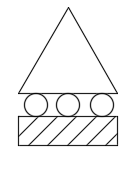
\includegraphics[width=2cm]{figuras/Capitulo_3/T1.png}   & Impede deslocamentos em ambas as direções.  \\
            \textbf{Móvel}  & 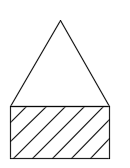
\includegraphics[width=2cm]{figuras/Capitulo_3/T2.png}   & Impede deslocamentos em apenas uma direção. \\
            \textbf{Engaste} & 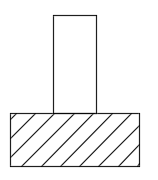
\includegraphics[width=2cm]{figuras/Capitulo_3/T3.png}  & Impede a rotação. \\
            \textbf{Mola}    & 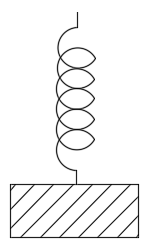
\includegraphics[width=2cm]{figuras/Capitulo_3/T4.png}  & Diminui a rigidez de translação do nó.  \\
            \textbf{Mola rotacional} & 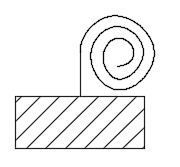
\includegraphics[width=2cm]{figuras/Capitulo_3/T5.png}  & Diminui a rigidez de rotação do nó.                 
        \end{tabular}
        \label{tab:3.1}
    \end{table}

\section{Métodos aproximados} 

\indent As soluções aproximadas para equações diferenciais satisfazem o equilíbrio em um sentido médio, não pontualmente em todas as 
coordenadas. Tais aproximações são tipicamente expandidas como uma combinação linear de um conjunto de funções de base ponderadas por 
parâmetros arbitrários \citet{finlayson1972method}. 

\subsection{Métodos dos resíduos ponderados}

\indent Os métodos dos resíduos ponderados englobam técnicas para a obtenção de soluções aproximadas de equações diferenciais lineares ou não 
lineares, servindo também como pilar matemático fundamental para formulações variacionais empregadas no Método dos Elementos Finitos (MEF) e 
o Método dos Elementos Virtuais (MEV). 

\indent Dado um operador diferencial $L$ e um termo de excitação de forças ou fontes $F$, a função resíduo surge da diferença entre a 
aplicação do operador sobre a solução aproximada $u_h$ e o termo exato $F$:

\begin{equation}
    R = L(u_h) - F.
    \label{eq:3.44}
\end{equation}

\indent Nesse escopo, a solução candidata é expandida usando um conjunto predefinido de funções teste (funções de aproximação) $\varphi_i$, 
ponderadas por coeficientes ou graus de liberdade ajustáveis $a_i$ que garantem a melhor aproximação possível \citet{hughes1987finite}: 

\begin{equation}
    u_h(\mathbf{x}) = \sum_{i=1}^n a_i \varphi_i(\mathbf{x}).
    \label{eq:3.45}
\end{equation}



\indent O algoritmo minimiza o resíduo da equação por intermédio da ortogonalização frente a um conjunto de funções peso $w_i$: 

\begin{equation}
    \int_{V} w_i R \, dV = 0, \hspace{1cm} i = 1,2,...,n.
    \label{eq:3.46}
\end{equation}



\indent Essa abordagem ramifica-se em diversas variantes, distinguindo-se primordialmente pela escolha da função peso. As metodologias 
estão sintetizadas na Tabela~\ref{tab:3.2}:

    
    \begin{table}[htbp]
        \caption{Tabela 3.2}
        \begin{tabular}{lll}                                                                                           \\
            \multicolumn{1}{c}{\textbf{Método}} & \multicolumn{1}{c}{\textbf{Função peso ($w_i$)}}                 & \multicolumn{1}{c}{\textbf{Ideia principal}}                         \\
            \textbf{Colocação}                  & Delta de Dirac $(w = \delta(x_j - x))$                           & Impõe $(R=0)$ em pontos específicos do domínio.                      \\
            \textbf{Subdomínios}                & $(w_i=1)$ em cada subdomínio e $(0)$ fora                        & Anula o resíduo em média em cada subdomínio.                         \\
            \textbf{Mínimos Quadrados}          & $(w_i=\dfrac{\partial R}{\partial a_i})$                         & Minimiza a norma quadrática do resíduo.                              \\
            \textbf{Galerkin}                   & $(w_i=\textbackslash{}varphi_i)$ (mesmas funções de aproximação) & Utiliza as mesmas funções para aproximação e ponderação.             \\
            \textbf{Petrov–Galerkin}            & $(w_i\neq varphi_i)$                                             & Utiliza funções de ponderação diferentes das funções de aproximação.
        \end{tabular}
        \label{tab:3.2}
    \end{table}


\indent De acordo com \citet{rao2017finite}, a formulação de Galerkin destaca-se por fornecer resultados altamente robustos em mecânica dos sólidos. Trata-se, historicamente, da rota mais percorrida para a derivação variacional das matrizes de elementos finitos. 

\indent Resolver a equação diferencial no seu formato "forte" (original) requer um elevado grau de regularidade (continuidade) da função aproximadora. A variável primária necessita ser diferenciável até a ordem máxima estipulada pelo operador analítico. A migração para a forma fraca, de natureza integral, relaxa drasticamente essa exigência. 

\subsection{Forma fraca da equação governante}

\indent Resgatando a equação de Cauchy Eq.~\ref{eq:3.18}, o resíduo exibe a seguinte forma: 

\begin{equation}
    R(u, \dot{u},\ddot{u}) = \nabla \cdot \mathsf{T}  +  b  -  \rho \ddot{u}.
    \label{eq:3.47}
\end{equation}


\indent O método de Galerkin exige que o resíduo seja ortogonal à cinemática admissível, representada por uma função peso $w$ genérica: 

\begin{equation}
    \int_{V} w (\nabla \cdot \mathsf{T}  +  b  -  \rho \ddot{u}) dV = 0.
    \label{eq:3.48}
\end{equation}


\indent Distribuindo a integral: 

\begin{equation}
    \int_{V} \nabla w \cdot \mathsf{T} \hspace{1.5pt} dV  + \int_{V} w \hspace{1.5pt} b \hspace{1.5pt} dV = \int_{V} w \hspace{1.5pt} \rho \hspace{1.5pt} \ddot{u} \hspace{1.5pt} dV. 
    \label{eq:3.49}
\end{equation}

\indent Utilizando uma identidade vetorial aplicável a divergentes para expandir a primeira parcela: 

\begin{equation}
    \int_{V} \nabla \cdot (\mathsf{T}  w) dV - \int_{V} \nabla w : \mathsf{T}  \, dV  + \int_{V} w \hspace{1.5pt} b \hspace{1.5pt} dV = \int_{V} w \hspace{1.5pt} \rho \hspace{1.5pt} \ddot{u} \hspace{1.5pt} dV.
    \label{eq:3.50}
\end{equation}

\indent O teorema da divergência atua estrategicamente para rebaixar a ordem derivativa na variável primal, transferindo-a simultaneamente 
para a função peso $w$. Adicionalmente, revela o termo de contorno que absorve as trações externas (condição de Neumann) de forma natural. 
Aplicando o teorema à Eq.~\ref{eq:3.50}: 

\begin{equation}
    \int_{V} w \hspace{1.5pt} \rho \hspace{1.5pt} \ddot{u} \hspace{1.5pt} dV + \int_{V} \nabla w : \mathsf{T}  \, dV  = \int_{V} w \hspace{1.5pt} b \hspace{1.5pt} dV + \int_{S} w \cdot \mathsf{t}^{(\hat{n})} \hspace{1.5pt} dS
    \label{eq:3.51}
\end{equation}

\indent O tensor gradiente do deslocamento virtual pode ser decomposto em sua componente simétrica (deformações) e antissimétrica (rotação 
rígida local): 

\begin{equation}
    \nabla w = \epsilon(w) + \tau(w).
    \label{eq:3.52}
\end{equation}

\indent Projetando-o sob o tensor de tensões via duplo produto escalar: 

\begin{equation}
    \nabla w : \mathsf{T}  = \left( \epsilon(w) + \tau(w) \right) : \mathsf{T}  = \epsilon(w) : \mathsf{T}  + \tau(w) : \mathsf{T}.
    \label{eq:3.53}
\end{equation}

\indent Como o tensor de tensões é inerentemente simétrico (equilíbrio de momento angular local), e a contração total de um tensor simétrico 
com um antissimétrico é nula, a igualdade reduz-se para: 

\begin{equation}
    \nabla w : \mathsf{T}  =  \epsilon(w) : \mathsf{T} .
    \label{eq:3.54}
\end{equation}

\indent Ao substituir a Eq.~\ref{eq:3.54} na Eq.~\ref{eq:3.51}, consolidamos a matriz da forma fraca: 

\begin{equation}
    \int_{V} w \hspace{1.5pt} \rho \hspace{1.5pt} \ddot{u} \hspace{1.5pt} dV + \int_{V}  \epsilon(w) : \mathsf{T}  \, dV  = \int_{V} w \hspace{1.5pt} b \hspace{1.5pt} d\Omega + \int_{S} w \cdot \mathsf{t}^{(\hat{n})} \hspace{1.5pt} dS.
    \label{eq:3.55}
\end{equation}

\indent Para que o termo dissipativo seja refletido, adota-se o modelo de Voigt, segregando o tensor em parcelas elástica e viscosa. 
Introduzindo a Eq.~\ref{eq:3.39} na Eq.~\ref{eq:3.55}: 

\begin{equation}
    \int_{V} w \hspace{1.5pt} \rho \hspace{1.5pt} \ddot{u} \hspace{1.5pt} dV + \int_{V}  \epsilon(w) : \mathbb{C} \epsilon(u) \hspace{1.5pt} dV + \int_{V}  \epsilon(w) : \mathbb{D} \dot{\epsilon}(u) \hspace{1.5pt} dV  = \int_{V} w \hspace{1.5pt} b \hspace{1.5pt} dV + \int_{S} w \cdot \mathsf{t}^{(\hat{n})} \hspace{1.5pt} dS
    \label{eq:3.56}
\end{equation}

\indent Ao mapear a base de sustentação contínua pelas matrizes de interpolação $\varphi$, a cinemática global recai no sistema algébrico: 

\begin{equation}
    \int_{\Omega} \rho \hspace{1.5pt} \varphi^T \hspace{1.5pt}  \varphi  \hspace{1.5pt} d\Omega \hspace{2pt} \ddot{u} + \int_{\Omega}  \epsilon(\varphi) : \mathbb{D} \epsilon(\varphi) \hspace{1.5pt} d\Omega \hspace{2pt} \dot{u} + \int_{\Omega}  \epsilon(\varphi) : \mathbb{C} \epsilon(\varphi) \hspace{1.5pt} d\Omega \hspace{2pt} u   = \int_{\Omega} \varphi \hspace{1.5pt} b \hspace{1.5pt} d\Omega + \int_{\Gamma} \varphi \cdot t^{(\hat{n})} \hspace{1.5pt} d\Gamma
    \label{eq:3.57}
\end{equation}

\indent A representação matricial condensada deste arcabouço dá origem à equação fundamental da dinâmica estrutural computacional: 

\begin{equation}
    [m] \ddot{u} + [c] \dot{u} + [k] u = f.
    \label{eq:3.58}
\end{equation}

\indent Uma escrita alternativa — muito popular em publicações matemáticas — utiliza o jargão de operadores bilineares para abstrair a forma 
fraca: 

\begin{equation}
    (w \hspace{1pt}, \hspace{1pt} \rho \ddot{u}) + a(w \hspace{1pt}, \hspace{1pt} \dot{u}) + a(w \hspace{1pt}, \hspace{1pt} u) = (w \hspace{1pt}, \hspace{1pt} b) + (w \hspace{1pt}, \hspace{1pt} \mathsf{t}^{(\hat{n})})_{S}
    \label{eq:3.59}
\end{equation}



\indent Os termos $a(\cdot,\cdot)$ e $(\cdot,\cdot)$ são exemplos de formas simétricas e bilineares. \\
\indent \citet{hughes1987finite} afirma que a notação utilizada na Eq.~\ref{eq:3.59} é concisa e captura aspectos matemáticos importantes. Devido a isso, essa 
notação será utilizada diversas vezes no decorrer dos próximos capítulos em definições.\\
\indent Para existir simetria, a seguinte propriedade deve ser cumprida:

\begin{equation}
    a(u,v) = a(v,u) \\ (u,v) = (v,u).
    \label{eq:3.60}
\end{equation}


\indent Do mesmo modo, para bilinearidade, dados dois coeficientes escalares $c_1$ e $c_2$:

\begin{equation}
    a(c_1 u + c_2 v, w) = c_1 a(u,w) + c_2 a(v,w) \\ (c_1 u + c_2 v, w) = c_1 (u,w) + c_2 (v,w).
    \label{eq:3.61}
\end{equation}

\subsubsection{Formulação fraca com análise modal para equação de vibração livre não amortecidas.}

\indent Sistemas operando em espectro livre e isento de atrito descartam imediatamente a parcela de carga transitória acoplada à matriz de 
dissipação: 

\begin{equation}
    [M]\ddot{u} + [K]u= 0 
    \label{eq:3.62}
\end{equation}

\indent Expressando o campo vetorial pelo somatório ortogonal, a premissa de repetição cíclica colapsa a equação para a verificação do 
problema de autovalor: 

\begin{equation}
    [K] -  \omega_n^2 [M])\phi_n = 0.
    \label{eq:3.63}
\end{equation}



\indent Essa equação contém a solução trivial $\phi_n = 0$, todavia isso implica a não existência de movimento, destarte a obtenção das 
frequências naturais e modos de vibração provêm da solução de um problema de autovalor.\\
\indent Ao aplicar o princípio da superposição modal à Eq.~\ref{eq:3.36}, o sistema de equações a ser resolvido é:

    \begin{equation}
        ([\Omega^2] -  \omega^2[I])\phi_n = 0.
        \label{eq:3.64}
    \end{equation}

\subsection{Método de Galerkin com discretização do domínio}

\indent Métodos numéricos tais como o MEF e o MEV utilizam a mesma estrutura que o método 
de Galerkin. Contudo, esses métodos subdividem o domínio em subdomínios chamados elementos e aplicam em cada elemento a formulação fraca, 
obtida do método dos resíduos ponderados.\\
\indent Os métodos com discretização do domínio buscam encontrar a solução de um problema complexo ao substituí-lo por um problema mais simples. 
Nesses métodos, divide-se a região de solução (o domínio) em sub-regiões menores interconectadas, chamadas de elementos. Os elementos são 
conectados entre si por meio de juntas denominadas nós ou pontos nodais. Como as variações das variáveis de campo no contínuo são 
desconhecidas, assume-se que a solução pode ser aproximada por funções simples, as quais são escritas em função do valor das variáveis de 
campo nos nós \citet{rao2017finite}. O problema torna-se, então, solucionar um sistema linear de equações cujas incógnitas são as variáveis de campo nodais.\\
\indent Esses métodos, mesmo sendo aproximados, apresentam a vantagem de a solução ser aprimorada com o aumento do poder computacional — 
prática chamada de refino. Existem tipos principais de métodos de refino, que podem ser aplicados em conjunto. O refino $h$, por meio da 
redução do tamanho dos elementos, aumenta a quantidade deles no objeto de análise. O refino $p$ aumenta a ordem das funções de aproximação. 
O refino $r$ melhora a solução ao mover os nós para regiões de alto erro, sem que haja aumento no número de nós ou elementos. Em alguns casos, 
pode ser necessário refazer a distribuição de elementos na malha. Destaca-se em \citet{rao2017finite} que, mesmo com o refino $h$, existe um limite em que a 
solução para de se aproximar da solução analítica da equação diferencial Figura~\ref{fig:11}

 \begin{figure}[htbp]
        \centering
        \caption{Curva de convergência do MEF.}
        
\includegraphics[width=\textwidth]{figuras/capitulo_3/11.png}
        \label{fig:11}
        {\small \textbf{Fonte:} [11]}
    \end{figure}

\indent O processo de solução desses métodos envolve uma sequência de etapas fixas, sendo elas:

\begin{enumerate}
    \item Discretização do domínio do problema em uma malha de elementos;
    \item adota-se uma interpolação adequada para o problema. A equação de aproximação deve ser simples do ponto de vista computacional e 
    satisfazer certos requisitos de convergência;
    \item derivam-se as matrizes e vetores elementares, tais quais as matrizes de rigidez e de massa, e os vetores de carga, seja utilizando 
    um princípio variacional apropriado, através do método dos resíduos ponderados ou baseando-se em condições de equilíbrio;
    \item unir as equações elementares em um sistema de equações global, como exemplo: $$[K] = \boldsymbol{\mathsf{A}}_{e=1}^{n_{el}} [k_e]$$
    \item solucionar o sistema de equações para obtenção das variáveis de campo, e
    \item computar outras variáveis através das variáveis de campo obtidas.
\end{enumerate}








        






               

   



   



    

     


              


               

   

     


\chapter{O método dos elementos virtuais}
% \include{XXX} % adicionar os .tex da pasta inputs

\postextual % a partir daqui são os elementos pós-textuais.
\bibliography{ref} % O alerta amarelo ("Empty `thebibliography' environment on input line 8.") é porque não há citações ainda
% \chapter{APÊNDICE}
% \chapter{anexo}
\end{document}
